Il pattern architetturale applicato alla componente server è la \textit{Layered Architecture}. \\
Si è scelto tale pattern in quanto la componente server risulta troppo complessa per essere destrutturata dovendo gestire i servizi di: anagrafica unità, anagrafica utente, gestione mappa, calcolo percorsi unità e gestione delle interfacce grafiche. Garantendo, poi, il principio di \glock{Separation of Concerns} tipico di tale architettura, diverse squadre potranno lavorare su diversi layer autonomamente.\\
Di seguito viene illustrato il diagramma dei package. Si noti che le dipendenze procedono in un'unica direzione senza creare cicli. Si noti, inoltre, che il sistema dipende dalla classe \textbf{Position} in ogni suo punto in quanto, trattando problematiche legate al movimento di un'unità in una griglia, avere un tipo di dato che rappresenti due coordinate cartesiane risulta particolarmente utile.

\begin{figure}[H]
	\centering
	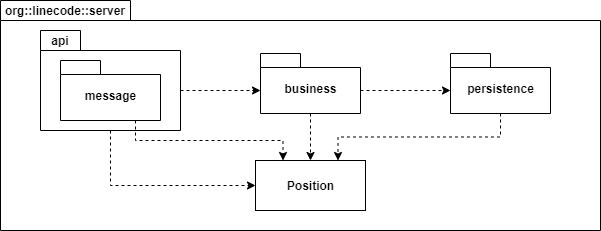
\includegraphics[width=12cm]{img/server_package.png}
	\caption{Server - Diagramma dei package}
\end{figure}

\begin{figure}[H]
    \centering
    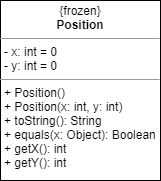
\includegraphics[width=4cm]{img/class_position.png}
    \caption{Server - Classe Position}
\end{figure}

\subsubsection{Messages}
Per garantire il principio \glock{Separation of Concerns}, è stato stabilito un formato standard di messaggi da e per UI e unità. Tali messaggi sono rappresentati come classi \glock{Java} e verranno scambiati con le altre componenti del prodotto in seguito alla loro serializzazione e deserializzazione in formato \glock{JSON} e oltre che venire scambiati internamente fra i vari layer in modo da garantire totale indipendenza dall'implementazione dei layer adiacenti.\\
Ogni messaggio viene riferito tramite la propria interfaccia in modo da slegare il sistema dall'implementazione di tali messaggi.

\begin{landscape}
    \begin{figure}[H]
        \centering
        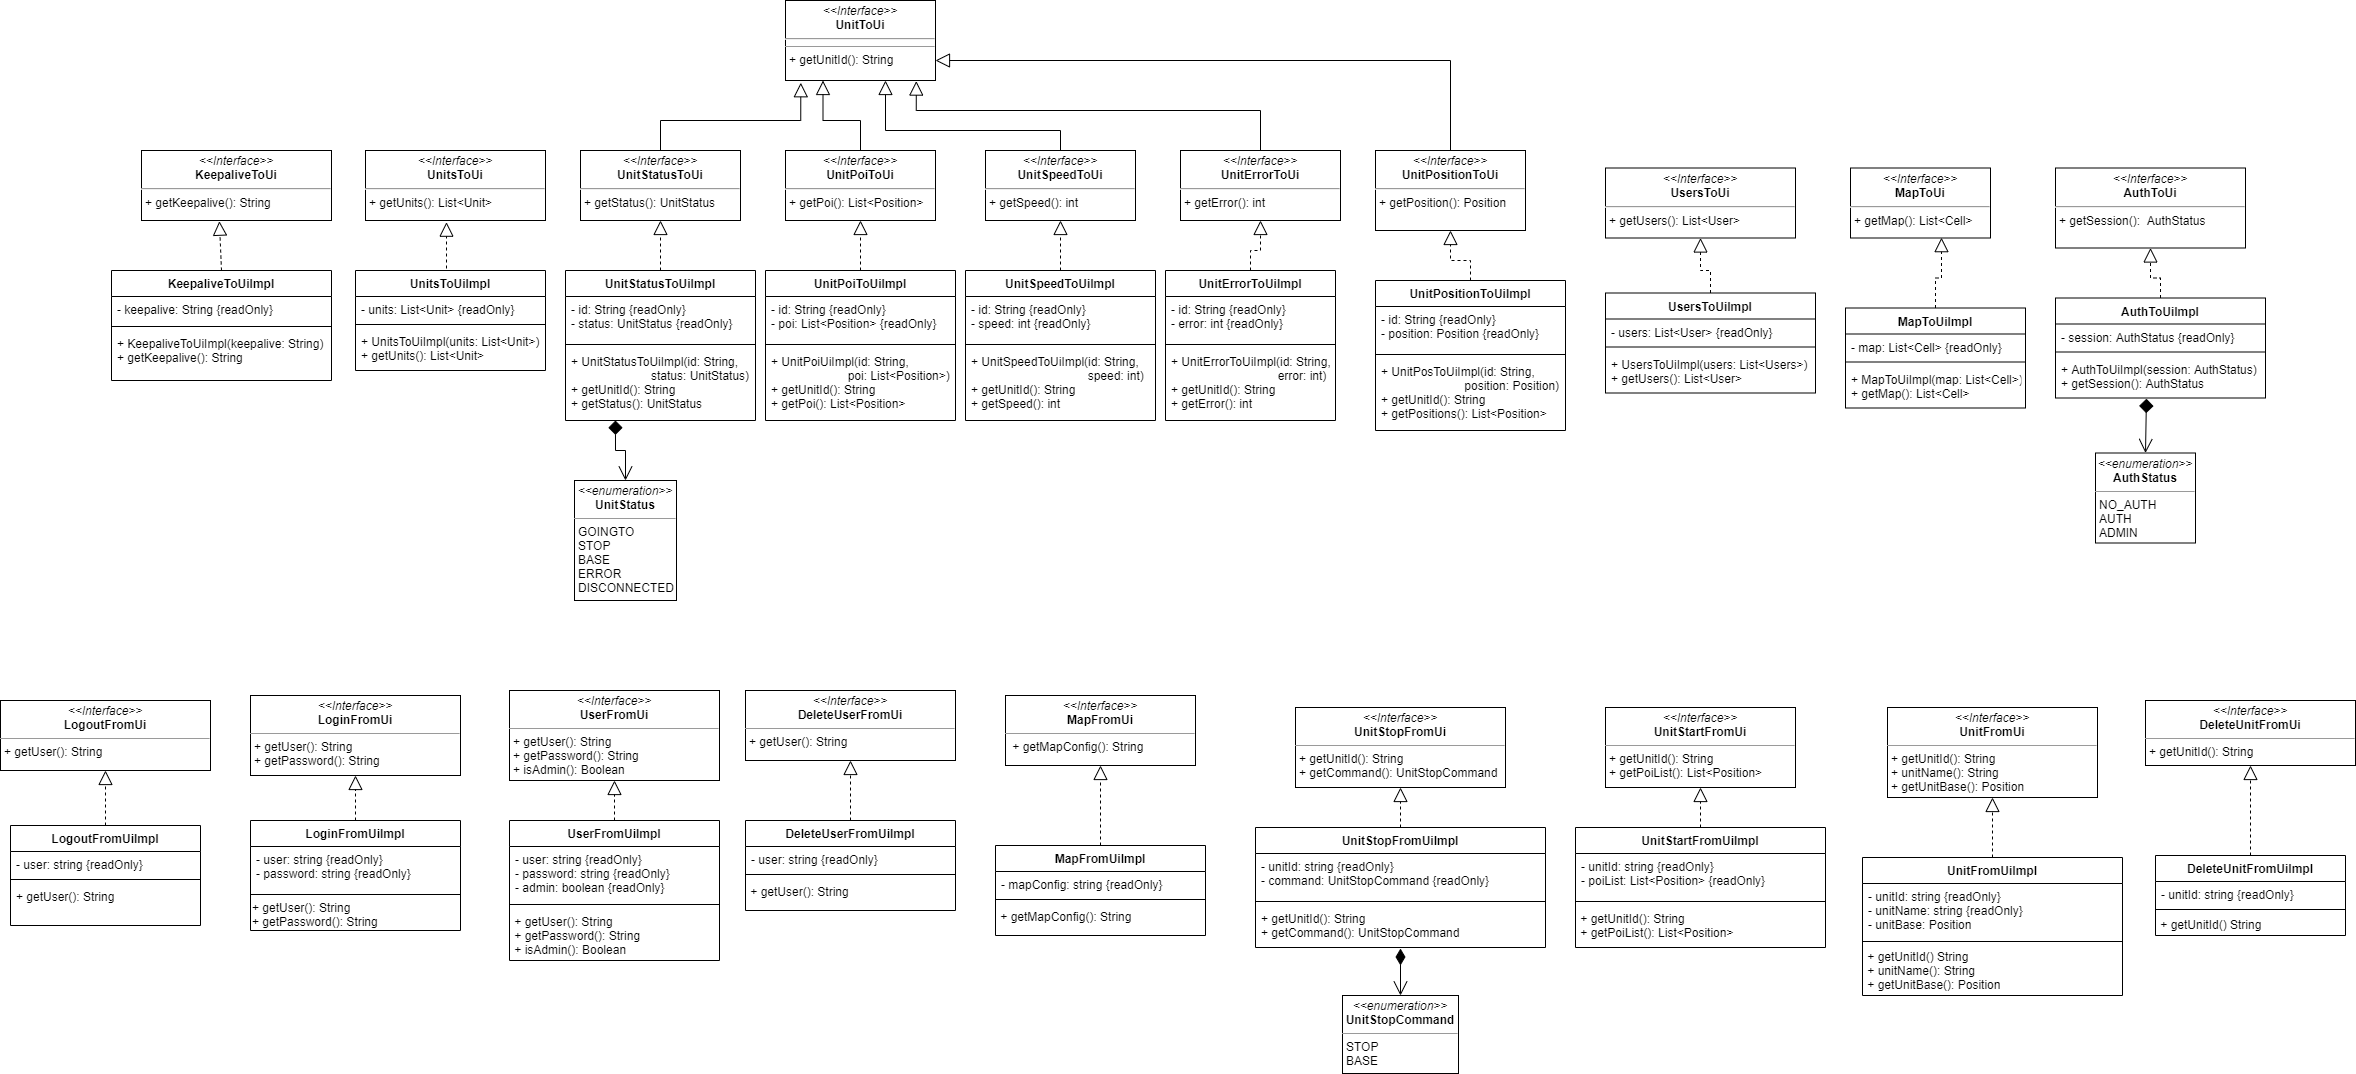
\includegraphics[width=24cm]{img/server_from_to_ui.png}
        \caption{Server - Messaggi da e per l'interfaccia}
    \end{figure}
\end{landscape}

\begin{landscape}
    \begin{figure}[H]
        \centering
        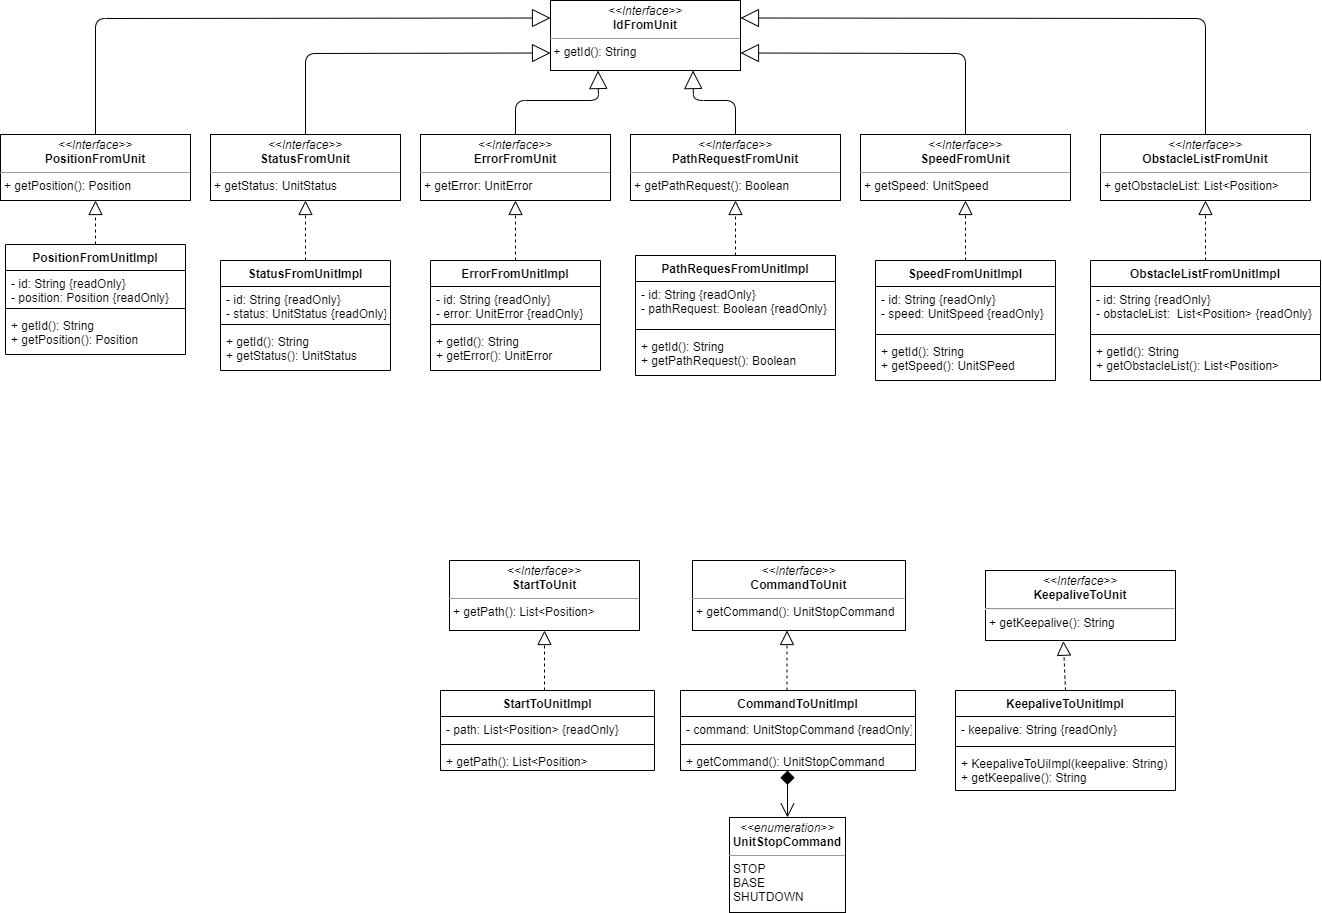
\includegraphics[width=24cm]{img/server_from_to_unit.png}
        \caption{Server - Messaggi da e per l'unità}
    \end{figure}
\end{landscape}

\subsubsection{API layer}
Qui troviamo i metodi che permettono la gestione della connessione alle altre componenti del sistema, e quindi anche l'invio e la ricezione di messaggi mediante opportune serializzazioni e deserializzazioni.

\subsubsection{Business layer}
Qui troviamo la logica per l'elaborazione dei dati in entrata ed uscita dal server.\\
Le informazioni scendono in questo layer tramite chiamata a funzione da parte dell'API layer su opportune interfacce. I prodotti dell'elaborazione vengono riportati nel layer superiore tramite oggetto ritornato dai metodi oppure, quando l'oggetto chiamante non è lo stesso che deve ricevere quanto ritornato, tramite l'emessione di opportuni segnali che verranno intercettati dal layer sovrastante secondo una logica \glock{signal/slot} simile alla libreria grafica \glock{Qt}. Lo slot viene consegnato tramite chiamata a funzione dall'API layer alla costruzione di un oggetto Endpoint in modo che possa avvenire la connessione fra segnale e slot. In tal modo viene messo in atto un sistema di scambio dei messaggi dal basso verso l'alto mantenendo la direzione delle dipendenze in senso contrario.

\subsubsection{Persistence layer}
Per immagazzinare i dati in uso all'applicazione, vengono utilizzate tre interfacce: anagrafica utenti ed anagrafica unità vengono implementate in \glock{SQLite}, mentre la struttura della mappa viene salvata in un file testuale opportunamente formattato.

\begin{landscape}
    \begin{figure}[h!]
        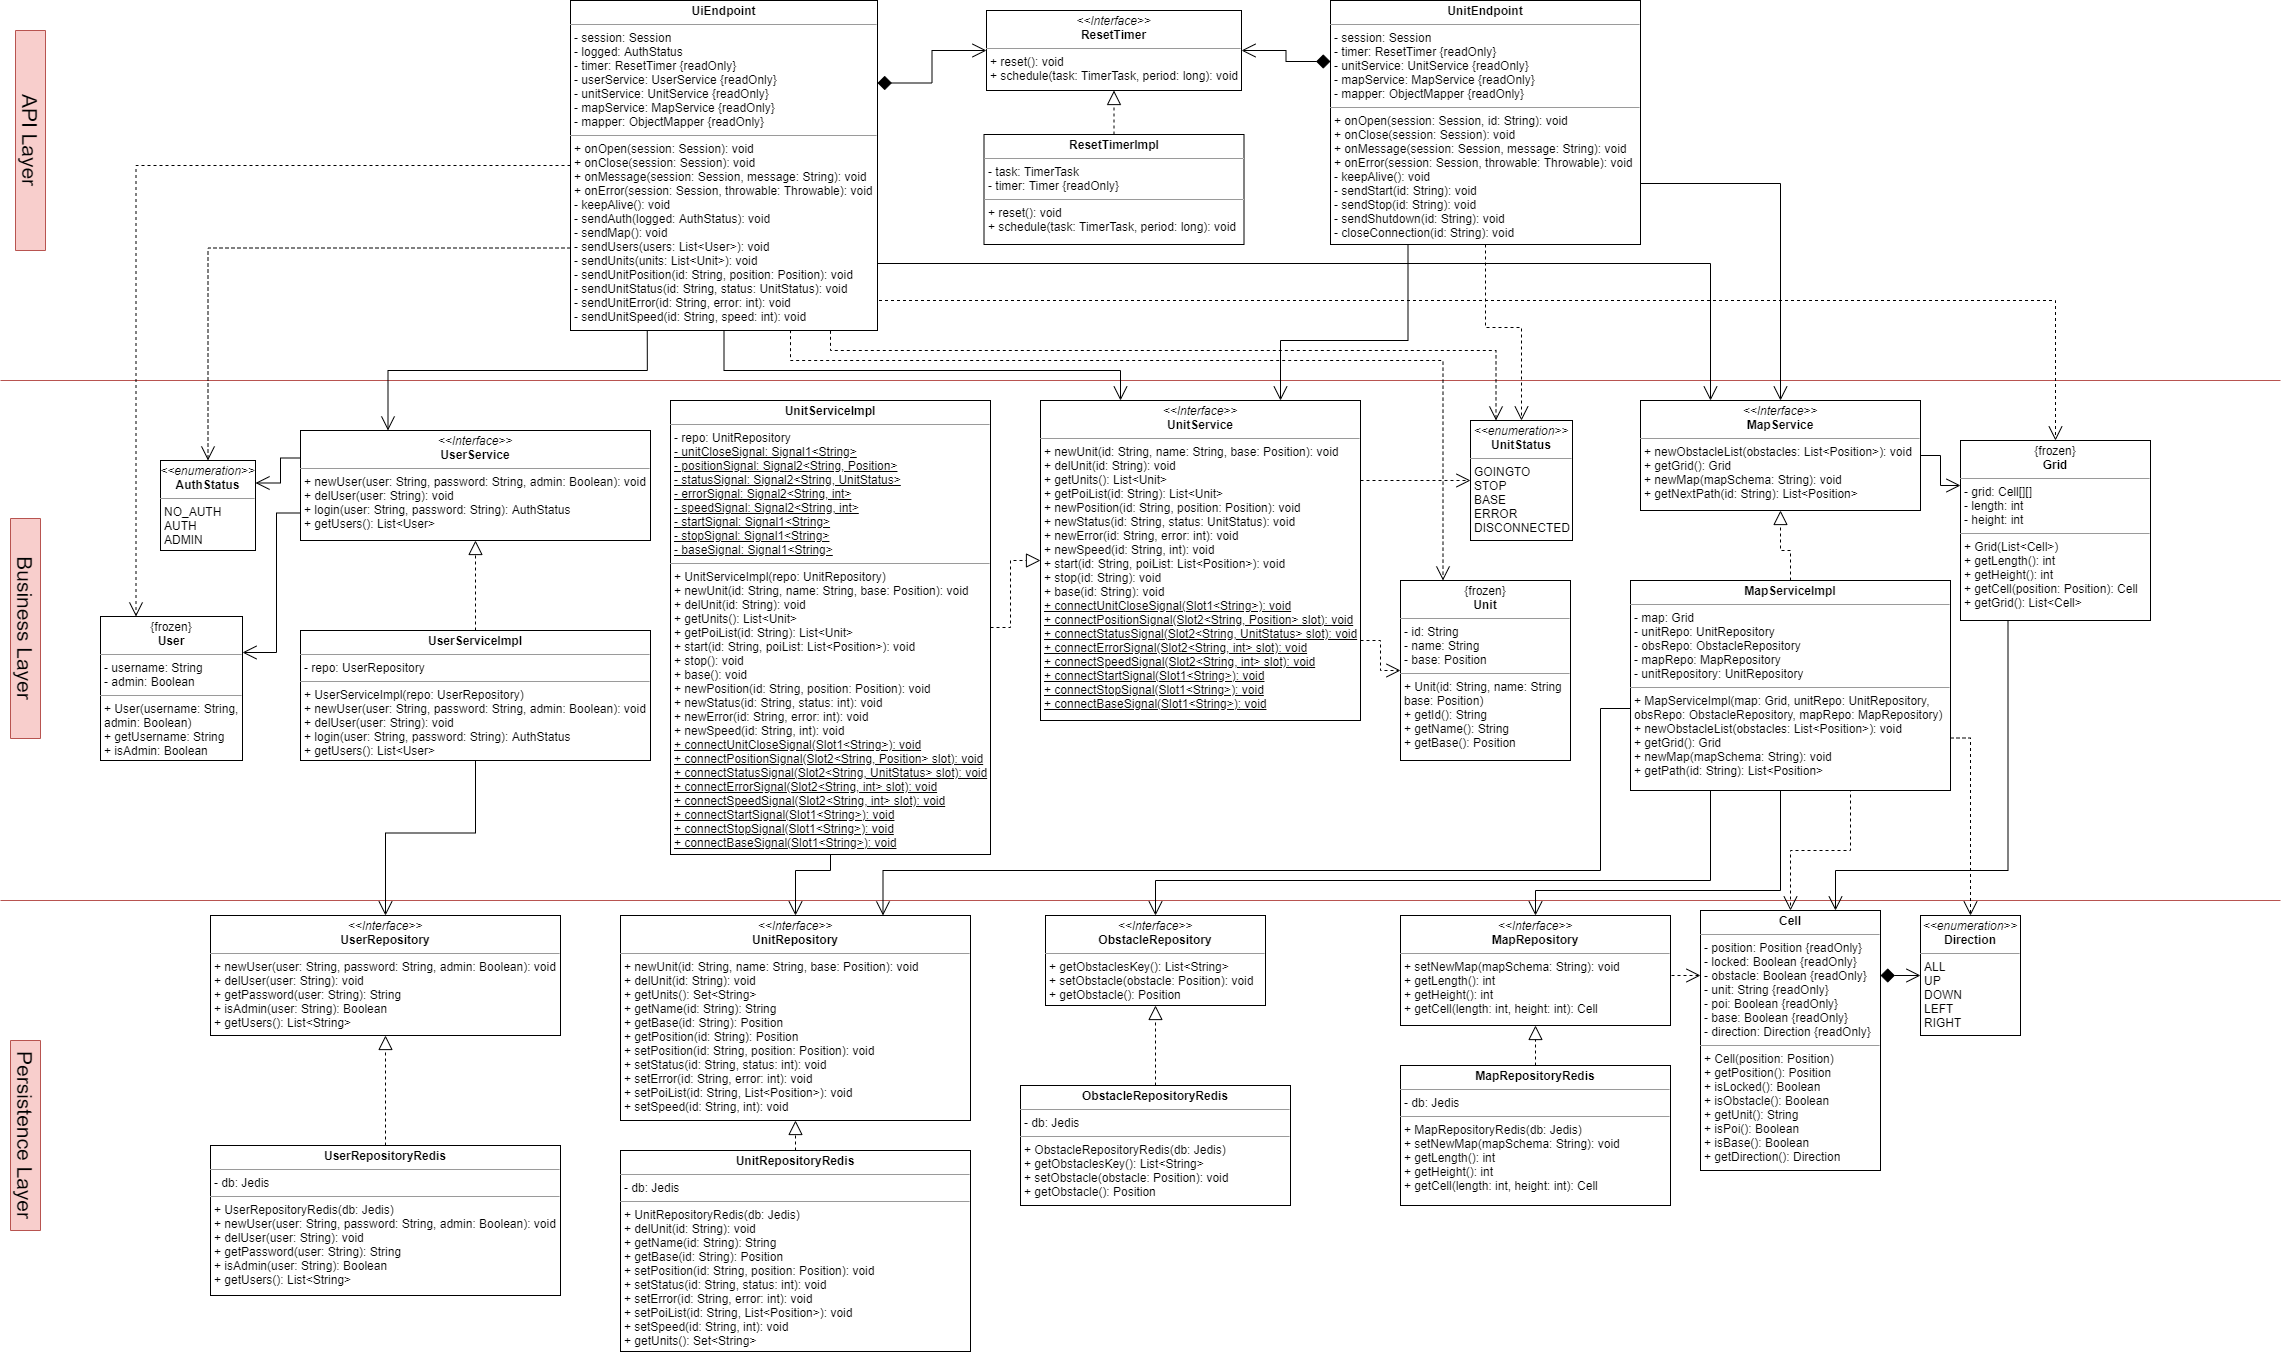
\includegraphics[width=26cm]{img/server_classi.png}
        \caption{Server - Diagramma delle classi}
    \end{figure}
\end{landscape}

\subsubsection{Database layer}
I dati che vengono immagazzinati nei file \glock{SQLite} possiedono la seguente struttura:
\begin{figure}[H]
	\centering
	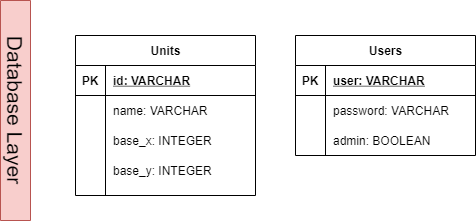
\includegraphics[width=10cm]{img/server_dblayer.png}
	\caption{Server - Database layer}
\end{figure}

\subsubsection{Diagrammi di sequenza}
Il seguente diagramma rappresenta il caso in cui l'interfaccia grafica invii al server una lista di \glock{POI}, che l'unità deve raggiungere.
\begin{figure}[H]
	\centering
	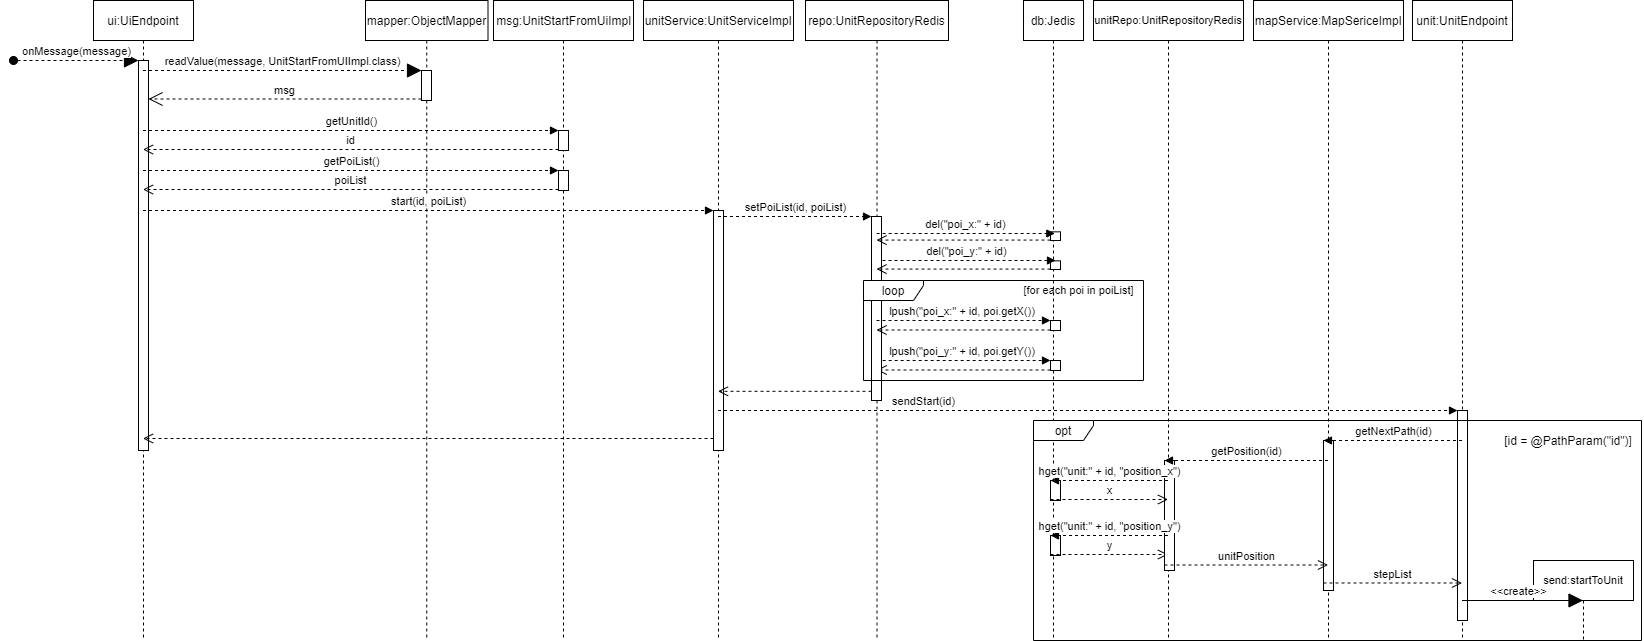
\includegraphics[width=16cm]{img/server_seq1.png}
	\caption{Server - UI invia una lista di \glock{POI} che l'unità deve raggiungere}
\end{figure}

\newpage
Il seguente diagramma rappresenta il caso in cui un utente esegua il login dall'interfaccia grafica.
\begin{figure}[H]
	\centering
	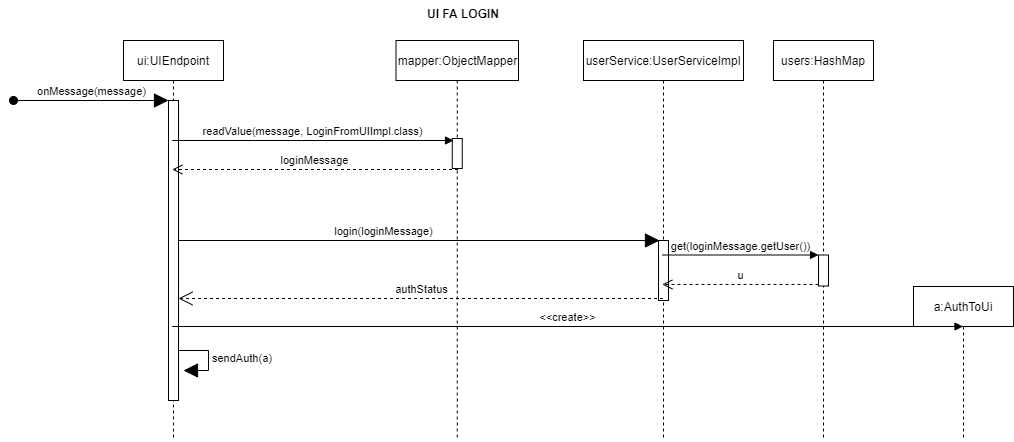
\includegraphics[width=16cm]{img/server_seq2.png}
	\caption{Server - Richiesta di login da parte della UI}
\end{figure}

Il seguente diagramma rappresenta il caso in cui un utente elimini un'unità registrata.
\begin{figure}[H]
	\centering
	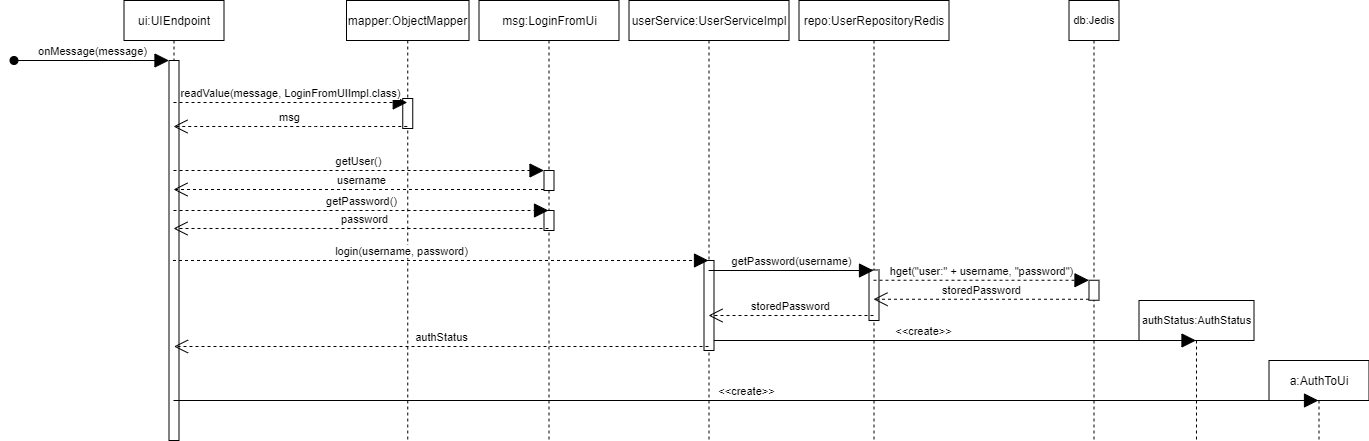
\includegraphics[width=16cm]{img/server_seq3.png}
	\caption{Server - UI richiede eliminazione unità}
\end{figure}